% BioBot-Rescue en una página. Compilar: pdflatex hoja.tex (las figuras las genera ../modelo/hoja.py)
\documentclass[10pt,letterpaper]{article}
\usepackage[spanish,es-tabla,es-noshorthands]{babel}
\usepackage[T1]{fontenc}
\usepackage[utf8]{inputenc}
\usepackage{lmodern}
\usepackage[margin=1.35cm,top=1.1cm,bottom=1.0cm]{geometry}
\usepackage{microtype}
\usepackage{graphicx}
\usepackage{array}
\usepackage{tabularx}
\usepackage{booktabs}
\usepackage{enumitem}
\usepackage[table]{xcolor}
\usepackage{multicol}
\definecolor{Primary}{HTML}{0E2A47}
\definecolor{Secondary}{HTML}{1D6FA5}
\definecolor{Accent}{HTML}{8A5200}
\definecolor{TableHead}{HTML}{D7E7F7}
\definecolor{SoftGray}{HTML}{F5F7FA}
\setlength{\parindent}{0pt}
\setlength{\parskip}{2.5pt}
\pagestyle{empty}
\setlist[itemize]{leftmargin=1.1em,itemsep=0pt,topsep=1pt,label=\textcolor{Secondary}{$\bullet$}}
\setlist[enumerate]{leftmargin=1.3em,itemsep=0pt,topsep=1pt}
\newcommand{\tit}[1]{\vspace{3pt}{\large\bfseries\color{Primary}#1}\par\vspace{-2pt}{\color{Secondary}\rule{\linewidth}{0.6pt}}\par\vspace{1pt}}
\renewcommand{\arraystretch}{1.08}

\begin{document}
\footnotesize
{\LARGE\bfseries\color{Primary}BioBot-Rescue en una página}\par
\vspace{1pt}
{\footnotesize\color{Primary}Sistemas Embebidos (O26-LRT3032-2) \,$\cdot$\, Roberto Orozco, Adam Del Pozo y Enrique Bernal \,$\cdot$\, 11 de noviembre de 2026}\par

\vspace{3pt}
\textbf{Qué es.} Una mochila electrónica de menos de 3~g sobre una cucaracha de Madagascar. El insecto
camina solo por los huecos de un derrumbe; la mochila detecta el calor de una persona, decide cuándo
darle un pequeño estímulo para que siga o gire, y avisa por radio cuando la encuentra.

\begin{multicols}{2}
\tit{Cómo funciona}
\begin{enumerate}
  \item \textbf{Ve.} Una matriz térmica de $8\times8$ mira al frente, diez veces por segundo.
  \item \textbf{Cuenta.} El circuito cuenta los píxeles «tibios»: entre 28 y 38~\textdegree C y
        2~\textdegree C sobre el fondo. Así no lo engañan ni un ambiente caluroso ni un objeto muy caliente.
  \item \textbf{Decide.} Una máquina de ocho estados deja que el insecto explore. Si se queda quieto
        15~s, le da un pulso; con 2 píxeles tibios lo gira hacia el calor.
  \item \textbf{Estimula poco.} Un LED ultravioleta junto a cada ojo, sin cirugía. Un presupuesto de 12
        estímulos acumulados obliga a descansar.
  \item \textbf{Avisa.} Con 8 píxeles durante cuatro cuadros seguidos declara la detección y manda la
        alerta por radio a un relevo en la entrada.
\end{enumerate}
\columnbreak
\tit{Por qué en FPGA}
La decisión completa ocupa \textbf{477 elementos lógicos}. Eso cabe en una FPGA de 1.4~mm y 2~mg, o
en un chip propio: lo único que el insecto carga sin esfuerzo es lógica. El mismo Verilog corre hoy en la
DE10-Lite y mañana en la mochila.

\tit{Qué se ha comprobado}
\begin{itemize}
  \item En simulación, el circuito coincide con su modelo de referencia en 11\,424 cuadros.
  \item Los cinco bancos de prueba pasan, incluido el de las dos tarjetas unidas por UART.
  \item \textbf{En una DE10-Lite real}, con el circuito y el insecto de prueba en el mismo chip: con una
        persona llega a ALERTAR en 7.4~s en modo rápido.
  \item \textbf{En dos DE10-Lite reales unidas por tres cables:} con una persona, la mochila pasa a
        acercar a los 26~s, cuenta 8 píxeles a los 54.6~s y alerta a los 55.1~s (la simulación da
        55.6~s). No alerta con el objeto caliente, sin persona ni con el insecto que no responde.
\end{itemize}
\end{multicols}

\vspace{-6pt}
\tit{Cómo se prueba hoy con dos DE10-Lite}
\begin{center}\vspace{-4pt}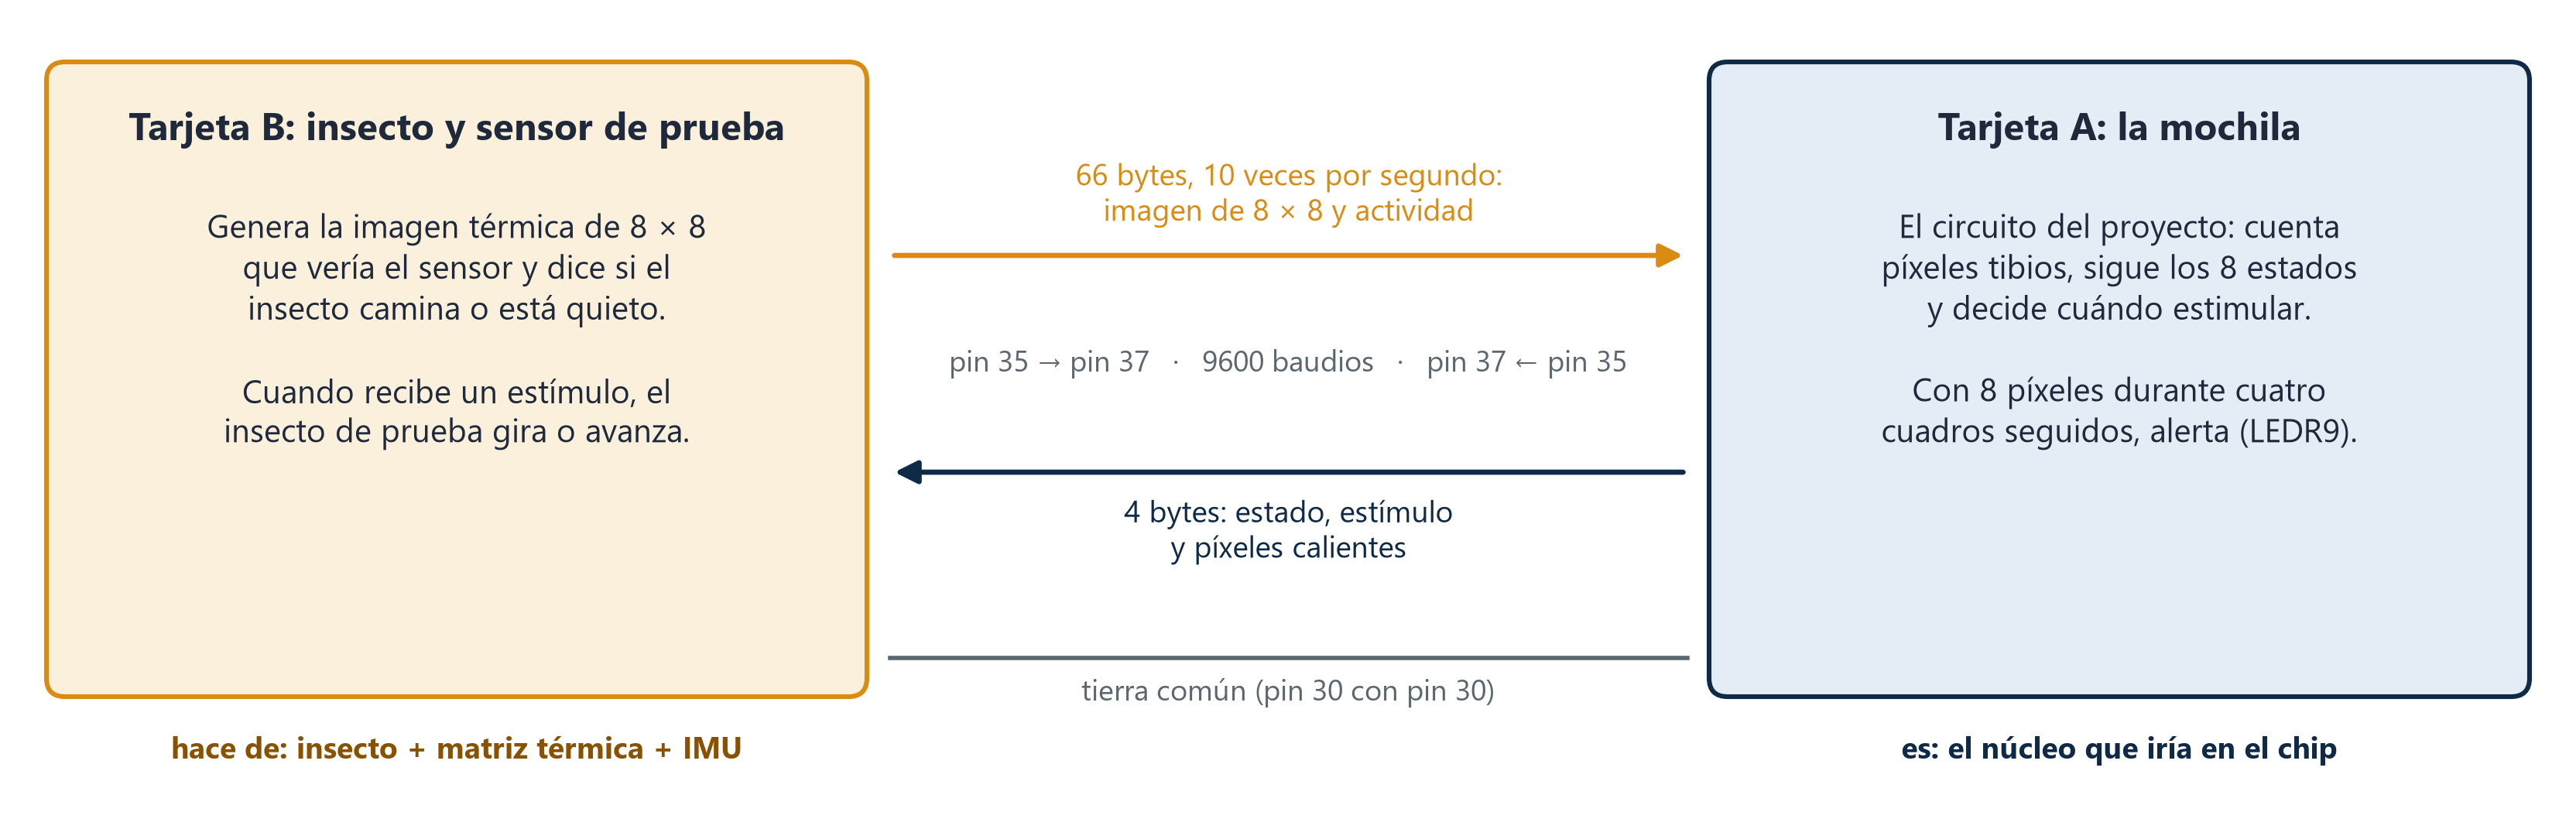
\includegraphics[width=0.80\linewidth]{figs/hoja_dos_tarjetas.png}\end{center}
\vspace{-8pt}
No hay insecto ni sensor en el laboratorio, así que una tarjeta hace de todo lo que rodea al circuito y la
otra es el circuito. Tres cables entre los conectores JP1: pin~35 con pin~37 en los dos sentidos y pin~30
con pin~30. En la tarjeta B se elige el escenario con SW2 y SW1 (01 = hay una persona); en la tarjeta A,
SW0 arranca la misión. Con una persona, HEX0 pasa de 1 (explorar) a 4 (acercar), 5 (confirmar) y 6
(alertar), y se enciende LEDR9 en cerca de un minuto. Con un objeto a 47.5~\textdegree C no debe alertar.

\tit{La mochila real: qué lleva, cuánto pesa y cuánto cuesta}
\begin{center}\vspace{-4pt}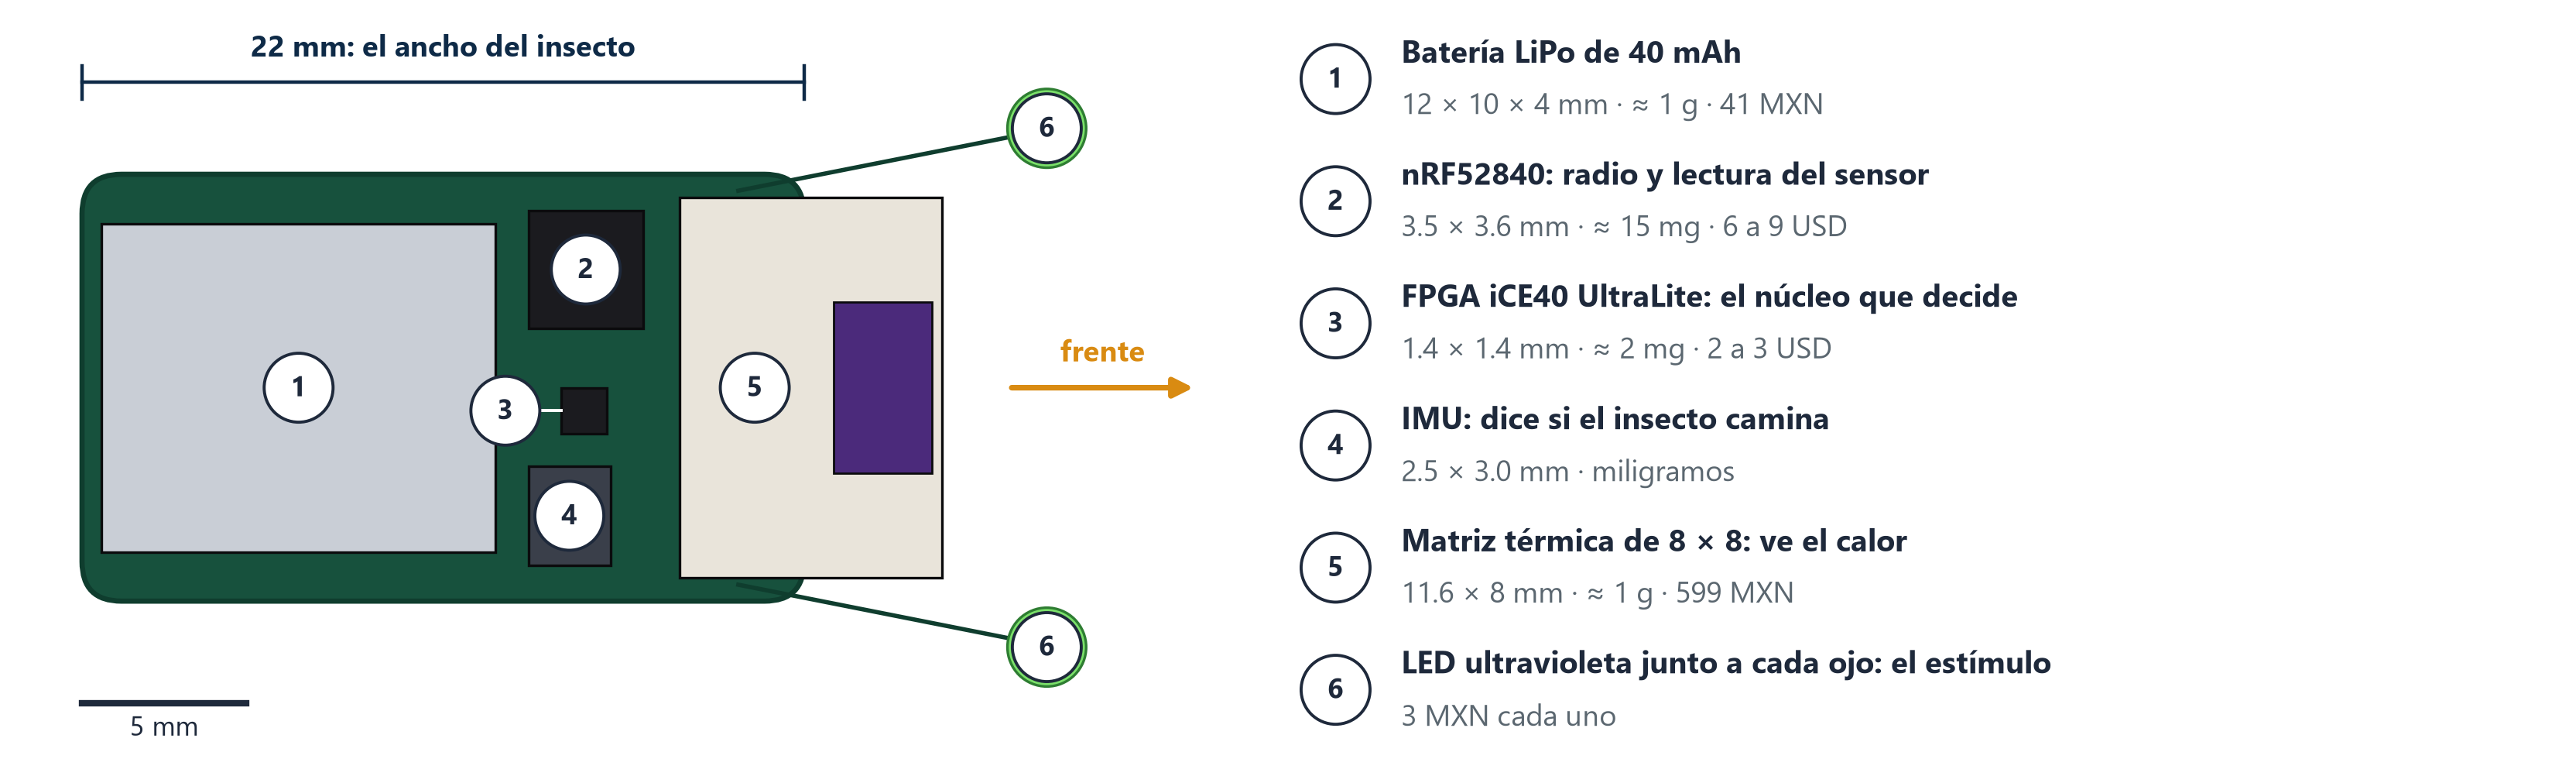
\includegraphics[width=0.90\linewidth]{figs/hoja_mochila.png}\end{center}
\vspace{-8pt}
\begin{tabularx}{\linewidth}{@{}>{\bfseries}l X >{\bfseries}l X@{}}
Peso total & 2.9~g: batería 1~g, sensor 1~g, tarjeta y chips 0.7~g, base 0.2~g. El insecto pesa 6.3~g y camina bien con 2 a 3~g &
Costo & Unos 950 a 1\,000~MXN en piezas (50 USD). Los dos chips, juntos, 8 a 12~USD \\
Autonomía & Unas 4~h con 40~mAh (consumo cercano a 30~mW; manda el sensor) &
Alcance & Empieza a acercarse a 1.3~m y confirma a 0.9~m de la persona \\
\end{tabularx}

\vspace{2pt}
{\footnotesize\color{Primary}\textbf{Lo que falta.} Soldar esos chips exige una tarjeta fabricada: no se montan a mano. Los precios de
los chips son de distribuidor y hay que confirmarlos. Para que los insectos vuelvan, en simulación un
refugio en la entrada recoge al 76~\% en dos horas y un faro infrarrojo que la mochila pueda seguir, al
91~\%: ninguno a todos, y con insectos no se ha probado. La ley mexicana solo permite manejar esta especie
en confinamiento.}
\end{document}
